\documentclass[10pt,a4paper,twocolumn,showkeys,showpacs,aps,groupedaddress,noeprint]{revtex4-1}
\usepackage[utf8]{inputenc}     % Atualmente é a codificação padrão
\usepackage[T1]{fontenc}
\usepackage{microtype}
\usepackage{graphicx}
\usepackage{subcaption}
\usepackage{ragged2e}
\DeclareCaptionJustification{justified}{\justifying}
\captionsetup{justification=justified,singlelinecheck=false,labelfont=large}

\usepackage{lipsum}% for dummy text

\begin{document}

\title{Título do artigo}
\author{Salviano de A. Leão}\email{salviano@ufg.br}
\affiliation{Instituto de Física,\\
Universidade Federal de Goiás,\\
C.P.131, 74.001-970,\\
Goiânia (GO), Brasil}
\author{João Ninguém}\email{joao.niquem@gmail.com}
\affiliation{Instituto de Física de Lugar Nenhum,\\
Universidade Federal de Lugar Nenhum,\\
C.P.777, 99.999-999,\\
Lugar Nenhum (XX), Brasil}
%\date{Novembro de 2009}

\begin{abstract}
   Aqui deve vir o resumo do seu trabalho. Você deve explicar
   de forma sucinta o que você fez
\end{abstract}

\keywords{Palavra-chave01, Palavra-chave02, Palavra-chave03}

\maketitle


\lipsum[1-3]

\begin{figure*}
        \begin{subfigure}[b]{0.485\textwidth}
           \centering
            \includegraphics[width=\textwidth,angle=-90]{Figs/fig1.eps}
            \label{fig:1}
\vspace{-12pt}
        \end{subfigure}
        \begin{subfigure}[b]{0.485\textwidth}
            \centering
            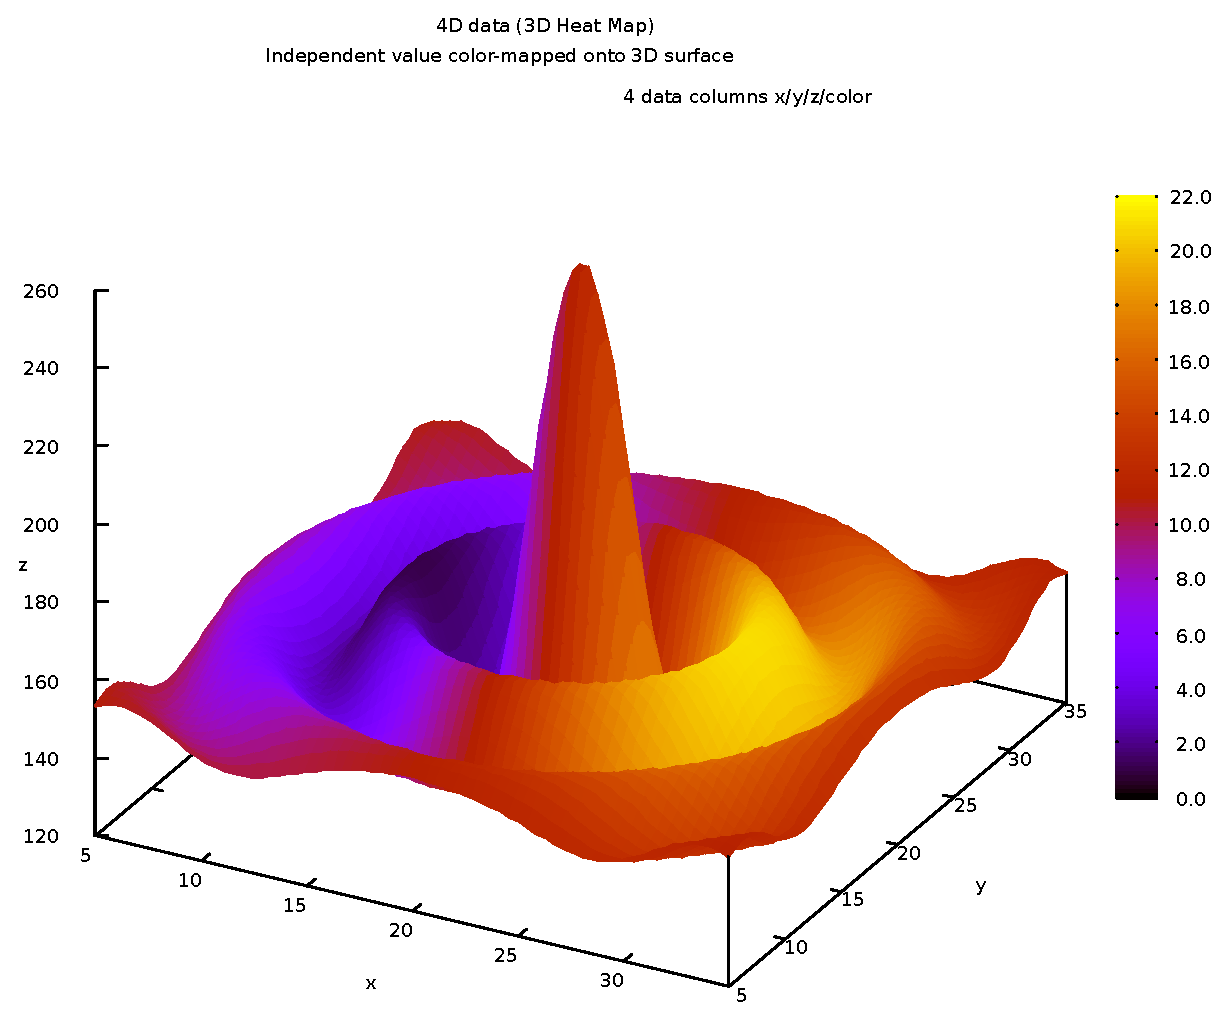
\includegraphics[width=\textwidth]{Figs/fig2.eps}
            \label{fig:2}
\vspace{-12pt}
        \end{subfigure}
 %       \vskip\baselineskip
        \begin{subfigure}[b]{0.485\textwidth}
            \centering
            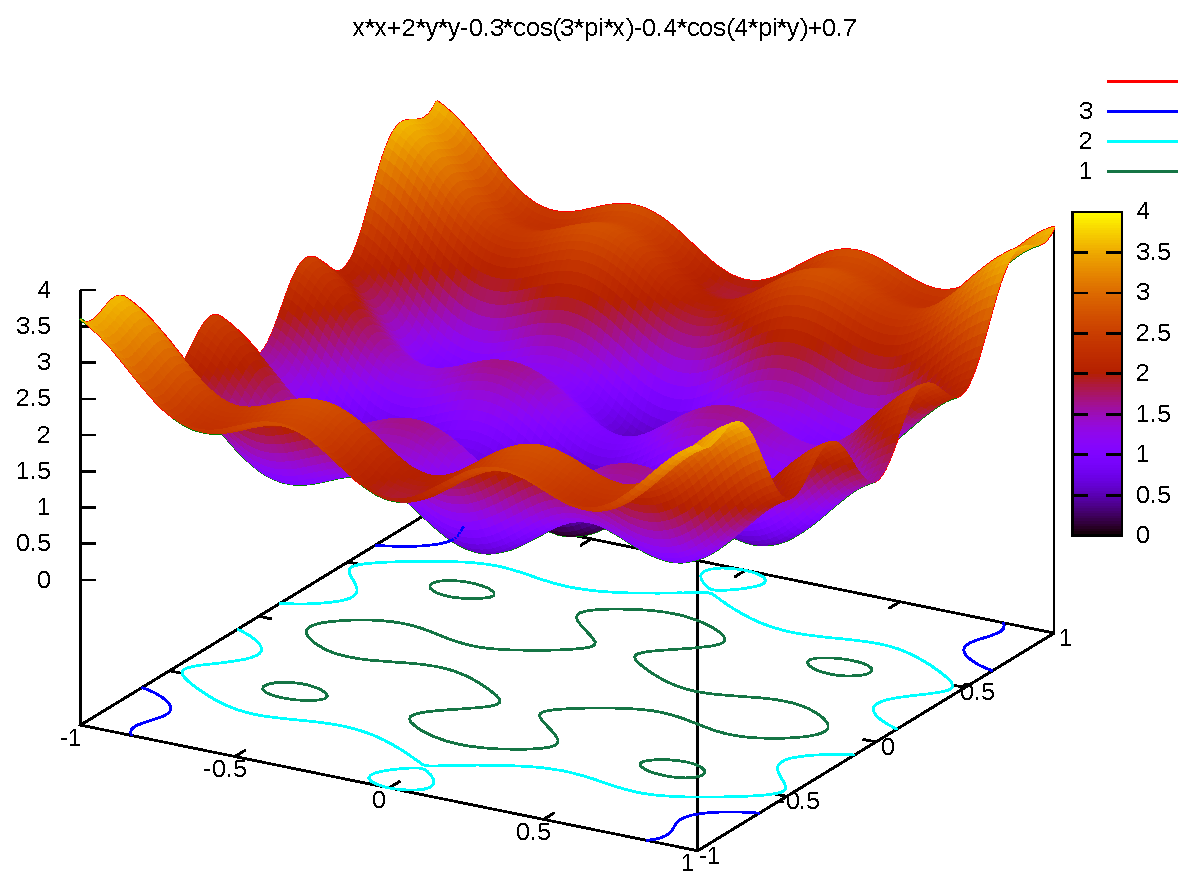
\includegraphics[width=\textwidth]{Figs/fig3.eps}
            \label{fig:3}
        \end{subfigure}
        \begin{subfigure}[b]{0.485\textwidth}
            \centering
            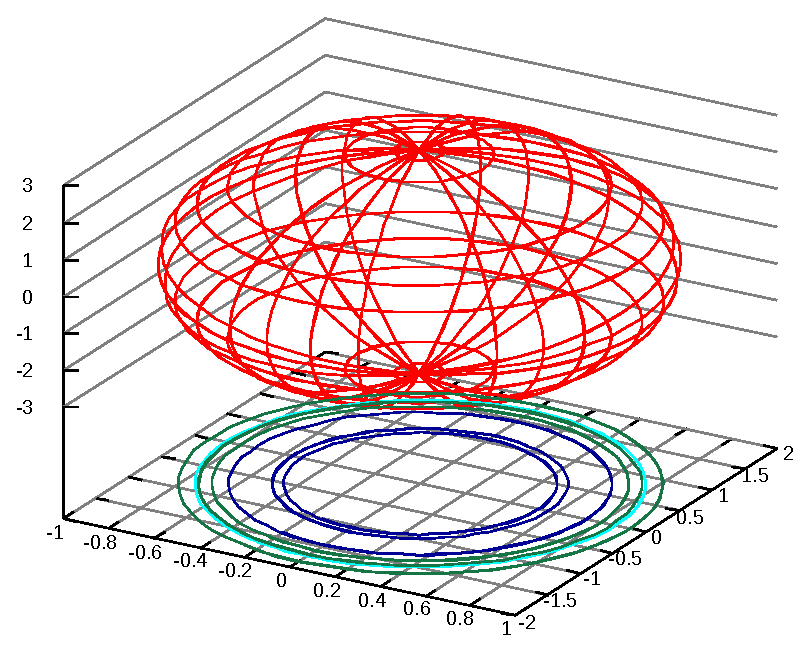
\includegraphics[width=\textwidth]{Figs/fig4.eps}
            \label{fig:4}
        \end{subfigure}
\vspace{-10pt}
        \caption[]{\small \lipsum[4]}
\label{fig:plot}
\end{figure*} 

\lipsum[4-7]
\end{document} 